\documentclass[11pt,a4paper]{article}
\usepackage[utf8]{inputenc}
\usepackage[T1]{fontenc}
\usepackage[polish]{babel}
\usepackage{lmodern}
\usepackage{graphicx}
\usepackage{epstopdf}
\usepackage{anysize}
\usepackage{makeidx}
\usepackage{hyperref}


\makeatletter
\renewcommand{\maketitle}{
\begin{titlepage}
\begin{center}

\LARGE{AKADEMIA GÓRNICZO-HUTNICZA}

\vspace*{1cm}

\includegraphics[scale=1.8]{agh.eps}
\vspace*{1cm}

\LARGE{im. Stanisława Staszica w Krakowie}

\rule{\textwidth}{0.4mm}
\LARGE \textsc{\@title}
\rule{\textwidth}{0.4mm}

\vspace*{5mm}


\large
\emph{Autorzy:}\\
Tomasz \textsc{Czarnik}\\
Konrad \textsc{Malawski}\\
Krzysztof \textsc{Śmiłek}\\

\vfill
\vspace*{\stretch{8}}
\rule{\textwidth}{0.4mm}

\large{Wydział Elektroniki, Automatyki, Informatyki i Elektrotechniki}\\
\large{Katedra Automatyki}\\
\vspace*{\stretch{7}}
\@date

\end{center}

\end{titlepage}
}
\makeatother

\title{Journey Diary}
\date{\today}

\makeindex

\begin{document}

\maketitle

\newpage

\tableofcontents

\newpage

\section {Sformułowanie zadania projektowego}
\subsection {Motywacja}
Journey Diary w zamierzeniu ma być aplikacją na system android, pozwalającą na dokumentowanie różnego rodzaju podróży (np. górskich wędrówek, tras rowerowych), która współpracowałaby z serwisem WWW. W serwisie tym użytkownicy mieliby możliwość prowadzenia podróżniczych blogów, dodawania zdjęć z podróży i zapisywania tras GPS.
	Na podstawie własnych doświadczeń zaobserwowaliśmy duże zapotrzebowanie na tego rodzaju usługę. W świetle rozkwitu różnego rodzaju serwisów społecznościowych, ludzie pragną dzielić się swoimi przeżyciami, także tymi z najróżniejszych podróży.
	Z początku aplikacja jak i usługa byłaby darmowa w celu zebrania jak największej liczby użytkowników. Następnie zakładamy wprowadzenie systemu inteligentnych, a zarazem przyjaznych użytkownikom promocji i reklam. Płatna, pełna wersja programu, udostępniałaby użytkownikom pełną funkcjonalność serwisu.

\subsection {Opis istniejących rozwiązań:}
Na rynku istnieje już wiele podobnych koncepcyjnie rozwiązań. Są to między innymi serwisy udostępniające użytkownikom możliwość prowadzenia dzienników podróży, ale także aplikacje dostępne na popularne platformy mobilne. Serwisy i aplikacje te są dedykowane aktywnym użytkownikom, którzy pragną dzielić się swoimi przeżyciami z innymi.

Z dostępnych rozwiązań należy wymienić kilka ciekawszych:
\begin{itemize}
\item blogipodroznicze.pl - serwisy pozwalające na dodanie własnej strony internetowej do bazy blogów o tematyce podróżniczej (katalog WWW);
\item geoblog.pl - umożliwia prowadzenie w ramach serwisu własnego bloga podróżniczego z możliwością dodania współrzędnych na mapie oraz zdjęć;
\item wojaze.net - możliwość dodania map, zdjęć i notatek z podróży;
\item Travel Blog - aplikacja na system Android umożliwiająca zapis na urządzeniu tras oraz notatek z podróży;
\item Travel Diary - jw. + możliwość dodania zdjęć i wsparcie dla facebooka;
\item My Trip Recorder - produkt najbliższy naszej koncepcji.
\end{itemize}

\subsection {Innowacyjność rozwiązania}
Proponowane przez nas rozwiązanie zakłada połączenie funkcjonalności konkurencyjnych rozwiązań, w szczególności ścisłej współpracy aplikacji z zewnętrznym, ogólnodostępnym, serwisem społecznościowym. Stawiamy na intuicyjność i prostotę interfejsu użytkownika oraz przyjemną oprawę wizualną. Z początku oferowane usługi nie przynosiłby zysku. W przypadku spopularyzowania produktu wierzymy, że mógłby on przynieść wymierny zysk.

\subsection {Obszar modelowania}

Projekt dzielimy na trzy współpracujące ze sobą części:
\begin{itemize}
\item Aplikacja kliencka - zainstalowana na telefonie użytkownika, umożliwia rejestrację trasy przy pomocy wbudowanego GPS, dodawanie notatek oraz zdjęć z podróży, a następnie synchronizuje pozyskane dane z serwisem;
\item Baza danych - przechowuje dane zgromadzone podczas wielu podróży, kolekcjonuje lokalizacje GPS oraz ścieżki dostępu do plików ze zdjęciami;
\item Aplikacja webowa - serwis umożliwiający przeglądniecie nadesłanych danych, ich modyfikacje i umieszczenie jako wpis w blogu podróżniczym, służy także za interfejs dla aplikacji klienckiej.
\end{itemize}

Ze względu na strukturę organizacyjną wyróżniamy następujące funkcje:
\begin{itemize}
\item Administrator systemu - zarządza bazą danych, moderuje użytkowników, może usuwać obraźliwe wpisy;
\item Redaktor - osoba, która korzysta z serwisu po zarejestrowaniu i zalogowaniu, może edytować podróże i umieszczać wpisy na blogu podróżniczym;
\item Użytkownik - posiada aplikację kliencką i dokonuje pomiarów GPS, wprowadza notatki i zdjęcia za pomocą telefonu;
\item Gość - nie wymaga rejestracji w serwisie, może jedynie przeglądać treści w nim zawarte i co najwyżej pozostawiać komentarze .
\end{itemize}

\section {Analiza funkcjonalności }

\subsection{Metoda MoSCoW}

Według metody MoSCoW, określa się następujące funkcjonalności aplikacji:

\subsubsection{Must - niezbędnę funkcjonalości:}
\begin{itemize}
\item Odczyt współrzędnych GPS
\item Możliwość dodania nowej podróży
\item Wykonanie zdjęcia
\item Dodanie notatki z podróży
\item Wysłanie zebranych danych do bazy serwisu (lokalizacja, zdjęcia, notatki)
\end{itemize}

\subsubsection{Should - funkcjonalności, które powinny zostać zrealizowane:}
\begin{itemize}
\item Dodanie geotaga do zdjęcia
\item Powiązanie notatki ze współrzędną
\item Upload danych na żądanie (minimalizacja kosztów transferu danych)
\item Minimalizacja użycia baterii poprzez automatyczne włączanie/wyłączanie odbiornika GPS
\end{itemize}

\subsubsection{Could - opcjonalne funkcjonalności:}
\begin{itemize}
\item Odczyt przybliżonej lokalizacji na podstawie nadajników GSM
\item Zapis trasy GPS jako plik formatu GPX
\item Ustawienie rozdzielczości wykonywanego zdjęcia
\end{itemize}

\subsubsection{Would - przyszłe plany rozbudowy:}
\begin{itemize}
\item Możliwość zapisywania i wysyłania sekwencji wideo
\item Integracja z innymi platformami
\end{itemize}

\subsection {Przepływy informacyjne doprowadzone do i wyprowadzane z systemu}
Przepływ informacji przedstawia poniższy diagram:\\
  \begin{figure}[h]
    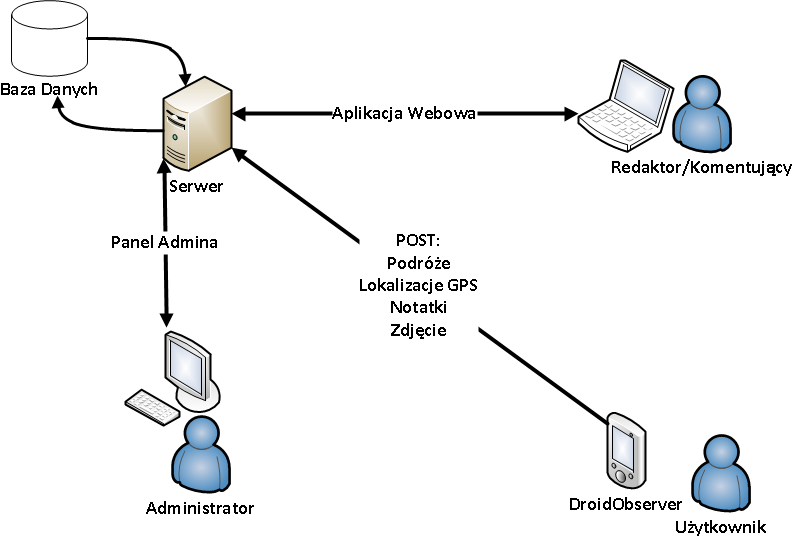
\includegraphics[scale=0.5]{data_flow.png}
    \caption{Przepływ informacji}
  \end{figure}

\subsection {Sygnalizowane specjalne wymagania i ograniczenia}
Zanim w ogóle rozpocznie się korzystanie z systemu należy podjąć kroki prawne regulujące zgodę użytkownika na przetwarzanie jego prywatnych danych w szczególności danych rejestacyjnych oraz położenia geograficznego. Aplikacja kliencka tworzona jest w Android API 8, a więc powinna poprawnie funkcjonować na urządzeniach działających pod kontrolą systemu operacyjnego Android 2.2 bądź kompatybilnych nowszych. Niezbędne do wysyłania informacji jest połączenie z Internetem, zalecamy wykupienie miesięcznego pakietu danych z nielimitowanym transferem (prędkość przesyłania danych nie jest specjalnie istotna), w przypadku braku połączenia internetowego aplikacja stara się kolekcjonować dane w celu ich wysłania na żądanie użytkownika. Urządzenie musi posiadać sprawny moduł GPS, najlepiej z opcją A-GPS pozwalającą na szybsze odnajdywanie pozycji satelitarnej.\\
\\
Dla potrzeb serwera wymagany jest serwer wspierający standard PHP 4 oraz baza danych PostgreSQL z wtyczką PostGIS. W celu dostępu do serwisu wystarczy dowolna przeglądarka internetowa, zalecamy użycie najnowszej wersji Chrome.

\section {Analiza systemu – diagramy UML}
\subsection {Diagram przypadków użycia systemu}
\begin{figure}[h]
    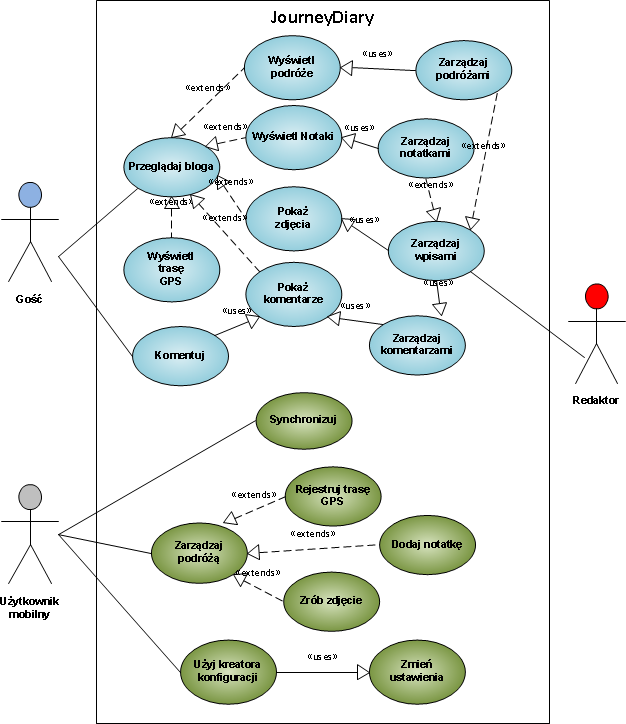
\includegraphics[scale=0.66]{use_case.png}
    \caption{Diagram przypadków użycia}
 \end{figure}
Na diagramie przypadki użycia po stronie serwera zaznaczono błękitnym kolorem, natomiast po stronie aplikacji klienckiej zielonym.

\newpage
%\subsection {Diagram klas systemu}
  %\begin{figure}[h]
  %  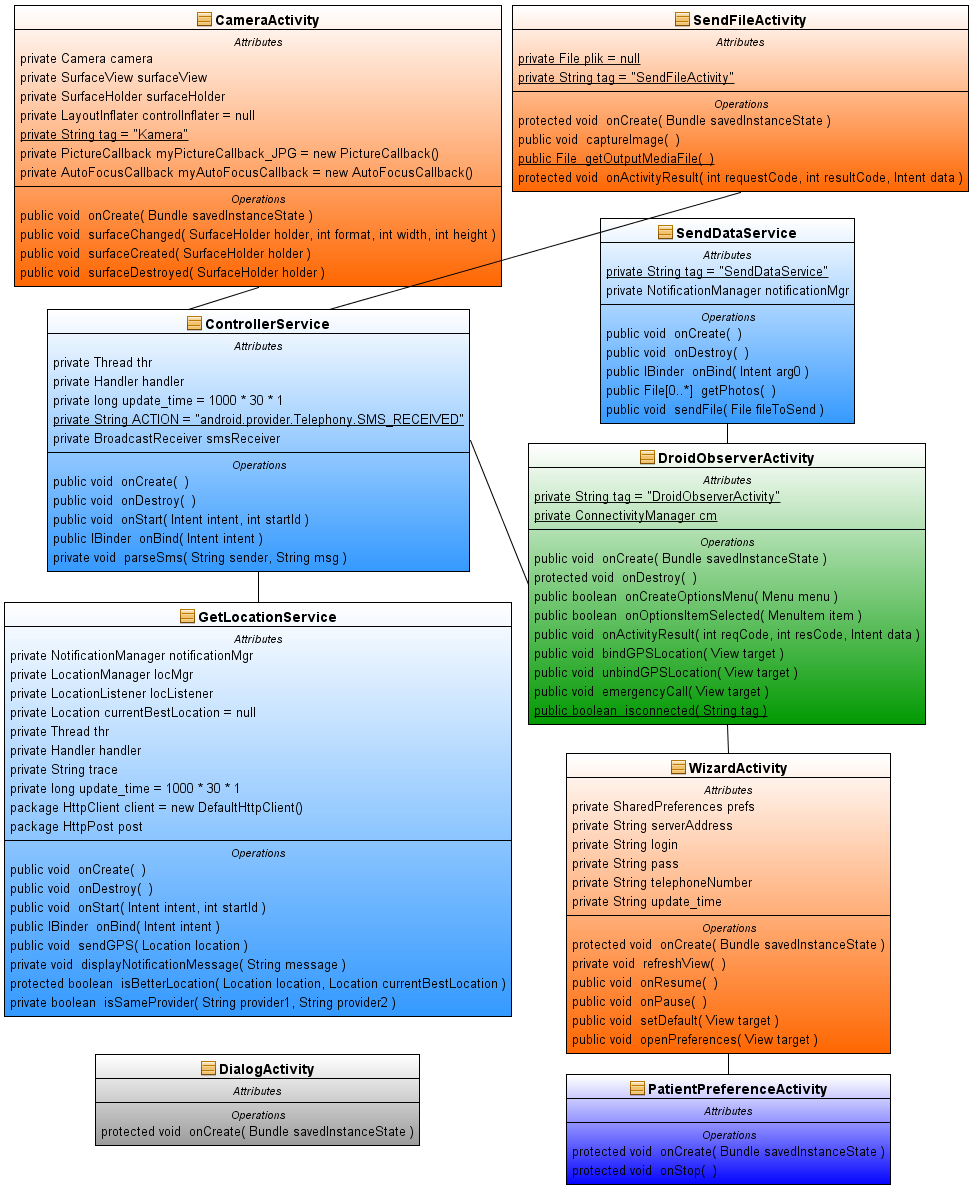
\includegraphics[scale=0.4]{class_diagram.png}
    %\caption{Diagram klas systemu}
  %\end{figure}
%Na rysunku przedstawiony został diagram klas systemu. Poszczególne kolory klas oznaczają:
%\begin{itemize}
%\item zielony - aktywność startowa (główna aktywność uruchamiana wraz ze startem aplikacji)
%\item błękitny - usługi: nie mają interfejsu, działają w tle
%\item pomarańczowy - zwykłe aktywności, posiadają interfejs
%\item szary - dialog, wyświetla małe szare okienko z informacją
%\item granatowy - aktywność preferencji
%\end{itemize}
\subsection {Diagram sekwencji}
\begin{figure}[h]
    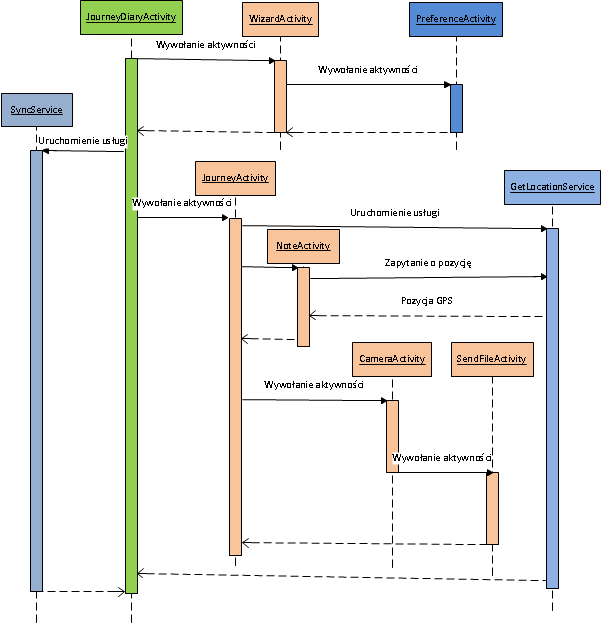
\includegraphics[scale=0.7]{sequence.png}
    \caption{Diagram sekwencji}
 \end{figure}
%Kolory analogiczne do diagramu klas.

\newpage
\subsection {Diagram najważniejszego stanu systemu}
\begin{figure}[ht]
    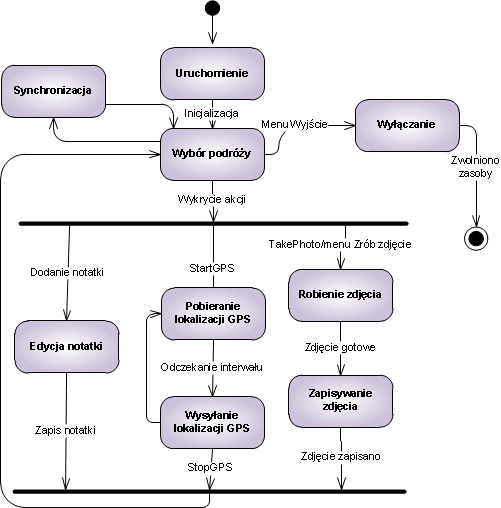
\includegraphics[scale=0.6]{state.png}
    \caption{Diagram stanu aplikacji JourneyDiary}
 \end{figure}
\subsection {Diagram Komponentów systemu}
\begin{figure}[ht]
    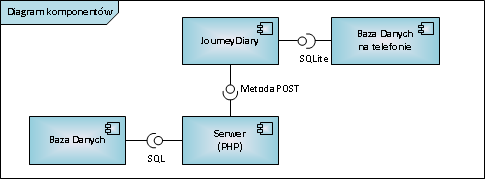
\includegraphics[scale=0.6]{component.png}
    \caption{Diagram komponentów}
 \end{figure}

\newpage
%\section {Instrukcja obsługi Systemu}
%\subsection{Instrukcja instalacji}
%
%\subsubsection{Instalacja aplikacji na telefonie}
%Plik JourneyDiary.apk wgrać na telefon z systemem Android 2.2 (lub wyższym) i uruchomić go.
%Instalacja powinna rozpocząć się automatycznie.
%
%\subsubsection{Instalacja bazy danych}
%\begin{enumerate}
%\item Założyc nową bazę danych
%\item W nowo stworzonej bazie danych uruchomić skrypt journeydiary.sql (plik ten znajduje się w folderze php) i zaobserwować czy powstały nowe tabele
%\end{enumerate}
%
%\subsubsection{Instalacja serwera}
%\begin{enumerate}
%\item Otworzyć plik config.php w edytorze tekstu
%\item Zmienić natępujące parametry według wzoru:
%\subitem \$baza = 'adres\_bazy\_danych';  (np. mysql.agh.edu.pl:3306);
%\subitem \$login = 'login\_do\_bazy\_danych'; 
%\subitem \$haslo = 'hasło\_do\_bazy\_danych';
%\subitem \$database\_name = 'nazwa\_bazy\_danych'
%\subitem \$admin\_login = 'login\_administratora'
%\subitem \$admin\_haslo = 'haslo\_administratora'
%\item Do katalogu public\_html (na serwerze) przegrać całą zawartośc folderu php
%\end{enumerate}
%
%\subsection{Instrukcja obsługi systemu}
%\subsubsection{Instrukcja obsługi serwisu WWW}
%
%Serwis WWW jest dostepny pod adresem:
%\begin{itemize}
%\item www.adresSerwera.domena - dla zwykłego użytkownika 
%\item www.adresSerwera.domena/admin.php - dla administratora systemu
%\end{itemize}
%
%{\bf Panel użytkownika}\\
%Aby skorzystać z panelu użytkownika należy zalogować się do systemu, poprzez podanie odpowiedniego loginu i hasła.
%Aby uzyskać dane dostępowe należy skontaktować się z admnistratorem systemu.
%Po zalogowaniu się użytkownik ma dostęp do nastepujących elementów:
%\begin{itemize}
%\item Przeglądanie aktualności (nie wymaga logowania się)
%\item Sprawdzanie swoich danych osobowych (Imię, Nazwisko, telefon, email, nazwa choroby)
%\item Odczytywanie ostatnich tras GPS 
%\subitem Po kliknięciu w daną datę otwiera się okno z wszystkimi trasami z danego dnia
%\item Przeglądanie zdjęć wysłanych na serwer
%\end{itemize}
%
%{\bf Panel administratora}\\
%Panel administratora poza standartowymi funkcjonalnościami umożliwia także:
%\begin{itemize}
%\item Dodawanie aktualności
%\item Dodawanie nowych pacjentów / Przeglądanie bazy wszystkich pacjentów
%\item Odczytywanie trad GPS każdego z pacjentów
%\item Przeglądanie zdjęć wyslanych przez konkretnego pacjenta
%\end{itemize}
%\vspace {20pt}
%\begin{figure}[h]
%\centering
%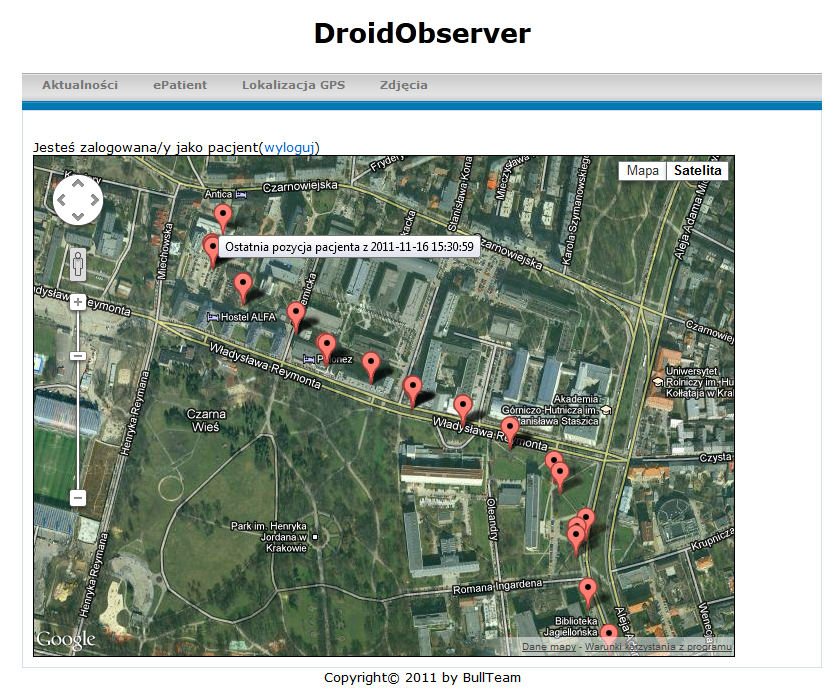
\includegraphics[scale=0.7]{route.png}   
%\caption {Wygląd trasy z panelu administratora}
%\end{figure}
%\vspace {20pt}
%
%\subsubsection{Instrukcja obsługi aplikacji}
%
%Po otwarciu nowo zainstalowanej aplikacji wyświetlony zostaje monit o podanie odpowiednich ustawień.
%Ich zmiany można dokonać także później poprzez wybranie z menu głównego opcji 'Ustawienia'.\\
%\\\\
%{\bf Widok opcji}
%\begin{enumerate}
%\item {\it Adres serwera*} - niezbędny do uzyskania połączenia (http://adresSerwera.domena/)
%\item {\it Login*} - unikalny login pacjenta
%\item {\it Hasło*} - używane do logowania na serwerze
%\item {\it Telefon alarmowy*} - Używany do połączen alarmowych
%\item Częstotliwośc odświeżania - Interwał pomiędzy kolejnymi wysyłanymi współrzędnymi
%\item Rozdzielczość aparatu - Rozdzielczość w jakiej robione będą zdjęcia
%\end{enumerate}
%
%* - pola unikalne (pozostałe opcje posiadają wartości domyślne)\\
%
%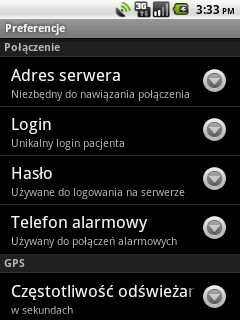
\includegraphics[scale=0.9]{screen_settings.png}    
%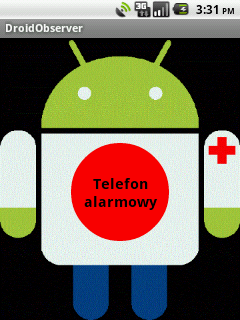
\includegraphics[scale=0.9]{screen_main.png}\\
%\\\\
%Po ustawieniu odpowiednich opcji nastepuje powrót do ekranu głównego. \\Można z niego wykonać jedną z poniższych opcji:
%\begin{itemize}
%\item Skontaktować się natychmiastowo z numerem alarmowym poprzez kliknięcie w duży czerwony przycisk na środku ekranu.
%\item Zrobic i wysłać zdjęcie na serwer  poprzez wybór odpowiedniej opcji z menu.
%\item Aktywować usługę wysyłania położenia GPS poprzez wybór odpowiedniej opcji z menu.
%\item Wyłączyć usługę wysyłanie położenia GPS  poprzez wybór odpowiedniej opcji z menu.
%\item Wyjść z programu poprzez wybór odpowiedniej opcji z menu.
%\end{itemize}
%
%\vspace{10pt}
%Aplikacja jest skonstruowana tak, by automatyzować pewne procesy. W szczególności umożliwia ona zdalne włączanie/wyłączanie odpowiednich opcji programu, poprzez analizę przychodzących SMSów. Jeśli aplikacja napotka na SMS z konkretną treścią uruchamia ona jedną z opcji programu. Oto lista obsługiwanych komend:
%\begin{enumerate}
%\item GetGPS - wysyła pod numer alarmowy SMSa z aktualną lokalizacją 
%\item StartGPS - uruchamia usługę wysyłania położenia GPS
%\item StopGPS - zatrzymuje usługę wysyłania położenia GPS
%\item TakePhoto - robi zdjęcie i wysyła na serwer
%\end{enumerate}
%\newpage
\section{Bibliografia}
Przy realizacji naszego projektu bardzo pomocne okazały się materiały dostarczone przez platformę IEEE
%\cite{2009UltraDeponti}
%\cite{2010ComputingEttinger}
\cite{2011IEEEIntGoldman}
\cite{2011IEEERadioMitchell}
%\cite{2009IEEEEngineeringSposaro}
\cite{2011DroidColunas}
%\cite{2010IEEEEMBCDoukas}
%\cite{2010IEEEEMBCSposaro}
%\cite{2009IEEEBIBEWang}
%\cite{2010NISSYang}.
Przy programowaniu na Androida nieocenione okazały się wskazówki zawarte w podręczniku 'Android 2. Tworzenie aplikacji'\cite{2010AndroidHashimi}.

\bibliographystyle{plain}
\bibliography{bibliography}

\end{document}
